 In this section, a labeled graph, called $(k,s)$-RdB graph, is used to represent $(k,s)$-RdB sequences. Just like a de Bruijn graph of order $k$, any simple path in $(k,s)$-Rdb graph represents a $(k,s)$-RdB sequence.

A $(k,s)$-RdB graph can be achieved by eliminating all the vertices containing more than $s$ consecutive letter $0$ in the de Bruijn graph $G_{k}$. As a result, the vertices of a $(k,s)$-RdB graph are represented by binary sequence of length $k-1$ which don't contain pattern $0^{s+1}$.

The illustration for de Bruijn graph of order $4$, $G_{4}$, was given in figure \ref{fig:dB4}. To obtain $(4,1)$-Rdb graph from there, vertices $000,001,100$ are deleted. Figure~\ref{fig:RdB_4_1} demonstrates the $(4,1)$-RdB graph.

\begin{figure}[htbp]
    \centering
    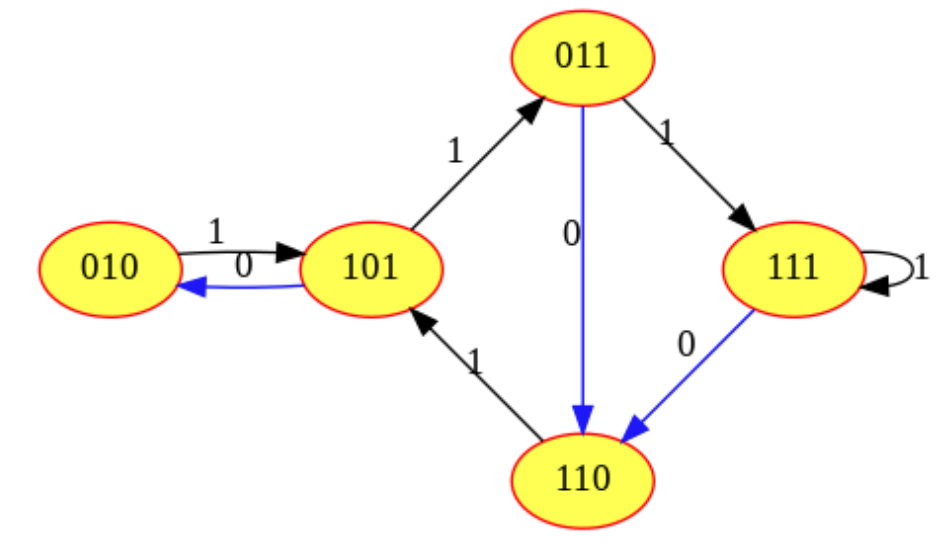
\includegraphics[scale=0.25]{fig/RdB41.png}
    \caption{$(4,1)$-RdB graph.}
    \label{fig:RdB_4_1}
\end{figure}

Denote the $(k,s)$-RdB graph to be $G_{k,s} = (V^{k-1,s},E^{k,s})$, where $V^{k-1,s}$ is the set of all vertices and $E^{k,s}$ is the set of all edges. The following lemmas determining the cardinality of $V^{k-1,s}$ and $E^{k,s}$

\begin{lemma}[\textbf{Number of vertices}]\label{lem:num_V}
    \begin{align}
        \card{ V^{k-1,s}} = \card{ W(k,s)}\label{eq:num_V}
    \end{align}
\end{lemma}
\begin{proof}
    This proof is deduced directly from the construction of $G_{k,s}$, since its set of all vertices is the set of all length $k-1$ sequences containing at most $s$ consecutive letters $0$. 
\end{proof}

\begin{lemma}[\textbf{Number of edges}]\label{lem:num_edges}
    \begin{align}
        \card{ E^{k,s}} = \card{ W(k,s)}\label{eq:card_of_E}
    \end{align}    
\end{lemma}
\begin{proof}
    Observe that for both $\bfx, \bfy\in W(k-1,s)$, if there is an edge from vertex $\bfx = (x_{1},\ldots,x_{k-1})$ to vertex $\bfy = y_{1},\ldots,y_{k-1}$, then $(x_{1},\ldots,x_{k-1},y_{k-1})\in W(k,s)$. 
    
    Besides, for each $s$-RLL sequence $\bfx=(x_{1},\ldots,x_{k})\in W(k,s)$, its prefix and suffix, $(x_{1},\ldots,x_{k-1})$ and $(x_{2},\ldots,x_{k})$, are both $s$-RLL sequence of length $k-1$. Hence, they represent two vertices in the graph $G_{k,s}$ and their connecting edge is represented by the sequence $\bfx$.
    
    So, there is $1-1$ correspondence between $E^{k,s}$ and $W(k,s)$. This results in $\card{ E^{k,s}} = \card{ W(k,s)}$.
\end{proof}

\begin{example}
    According to lemma \ref{lem:num_V} and lemma~\ref{lem:num_edges}, $(4,1)$-RdB graph has $\card{V^{3,1}}=\card{W(3,1)}=5$, and $\card{E^{4,1}} = \card{W(4,1)}=8$. These results can be verified by counting the number of vertices and edges in figure~\ref{fig:RdB_4_1}.
    % Applying lemma \ref{lem:num_V} and lemma~\ref{lem:num_edges} for $k=4,s=1$ gives $\card{V^{3,1}}=\card{W(3,1)}=5$, and $\card{E^{4,1}} = \card{W(4,1)}=8$. Counting the number of edges and vertices in figure~\ref{fig:RdB_4_1} provides the same results
\end{example}

Let $u=(u_{1},u_{2},\ldots,u_{k-1})$ and $v=(v_{1},v_{2},\ldots,v_{k-1})$ be arbitrary vertices in RdB graph. Starting at $v$, the following sequence of edges' labels $(1,u_{1},u_{2},\ldots,u_{k-1})$ apparently forms a proper path going from $v$ to $u$ in RdB graph. Similarly, the sequence of edges' labels $(1,v_{1},v_{2},\ldots,v_{k-1})$ beginning at $u$ is also a directed path from $u$ to $v$. This is sufficient to conclude that the connectivity of RdB graphs is preserved.
